\documentclass[UTF8, a4paper]{article}
\usepackage{ctex}
\usepackage{graphicx}
\usepackage[margin=2.5cm]{geometry}
\usepackage{subcaption}
\usepackage{amssymb}
\usepackage{amsthm}
\usepackage{amsmath}
\usepackage{enumerate}
\usepackage[backend=bibtex, style=alphabetic]{biblatex}
\usepackage{framed}
\usepackage{mathrsfs} 
\usepackage{xcolor}
\newtheorem{exercise}{Exercise \#14.}
\newtheorem*{proposition}{命题}
\newtheorem*{remark}{注}
\everymath{\displaystyle}

% \addbibresource{my.bib}
\title{Chapter 13\&14: 特征函数}
\author{}
\date{Latest Update: \today}
\begin{document}
\maketitle

\begin{framed}
\begin{exercise}
设\(X\)的pdf, \(f(x) = \frac{1}{\pi(1+x^2)}\)是一个Cauchy密度函数.
证明: 
$$
\varphi_X(u)=e^{-|u|},
$$
通过对以\([-R, R]\)为直径的半圆围线积分.
\end{exercise}
\end{framed}

\begin{proof}
\(X\)的特征函数为
$$
\varphi_X(t) = \mathbb{E}\{e^{itX}\} = \int_{-\infty}^{\infty} e^{itx} \frac{1}{\pi(1+x^2)} dx = \frac{1}{\pi} \int_{-\infty}^{\infty} \frac{e^{itx}}{1+x^2} dx.
$$
接下来, 求积分
$$
\int_{-\infty}^{\infty} \frac{e^{itx}}{(x - i)(x + i)} dx.
$$
显然, \(z = \pm i\)是被积函数的两个一阶奇点.

考察以下路径: 沿着实直线从\(-a\)到\(a\), 然后再依逆时针方向沿着以\(0\)为中心的半圆从\(a\)到\(-a\). 取\(a\)为大于\(1\), 使得虚数单位\(i\)包围在曲线里面, 如图所示.
\begin{figure}[htbp]
\centering
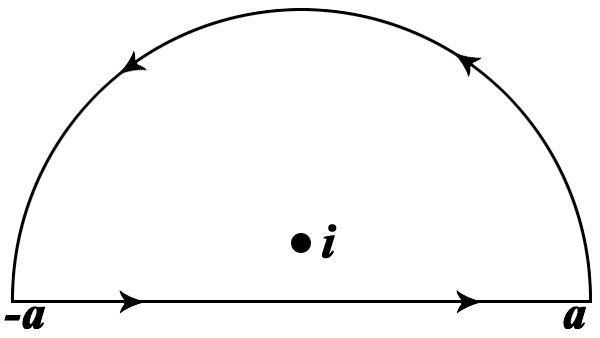
\includegraphics[width=0.5\textwidth]{ContourDiagram.png}
\end{figure}

路径积分为:
$$
{\displaystyle \int _{C}{f(z)}\,dz=\int _{C}{e^{itz} \over z^{2}+1}\,dz.}
$$
由于\(e^{itz}\)是一个整函数, 只有奇点\(z = i\)在路径\(C\)内部, 
根据一阶奇点留数公式, \({\displaystyle \operatorname {Res} (f,c)=\lim _{z\to c}(z-c)f(z).}\)
$$
\begin{aligned}
\frac{e^{i t z}}{z^2+1} & =\frac{e^{i t z}}{2 i}\left(\frac{1}{z-i}-\frac{1}{z+i}\right) \\
& =\frac{e^{i t z}}{2 i} \frac{1}{z-i}-\frac{e^{i t z}}{2 i(z+i)}
\end{aligned}
$$
于是留数是
$$
{\displaystyle \operatorname {Res} _{z=i}f(z)={e^{-t} \over 2i}.}
$$
根据留数定理, 
$$
{\displaystyle \int _{C}f(z)\,dz=2\pi i\cdot \operatorname {Res} _{z=i}f(z)=2\pi i{e^{-t} \over 2i}=\pi e^{-t}.}
$$
对路径积分做如下的分解, 
$$
{\displaystyle \int _{\mbox{straight}}+\int _{\mbox{arc}}=\pi e^{-t}\,}
$$
因此, 
$$
{\displaystyle \int _{-a}^{a}=\pi e^{-t}-\int _{\mbox{arc}}.}
$$
取极坐标参数化, 令\(z = Re^{i\theta}\), 其中\(\theta \in [0, \pi]\), 于是当\(t> 0\)时, 
$$
\begin{aligned}
\int _{\mbox{arc}} & \leq\int _{0}^{\pi}  \frac{R}{R^2 - 1}  \,d\theta \\
& = \frac{\pi R}{R^2 - 1} \to 0, \quad \text{当} R \to \infty.
\end{aligned}
$$
于是 
$$
{\displaystyle \int _{-\infty }^{\infty }{e^{itz} \over z^{2}+1}\,dz=\pi e^{-t}.}
$$

当\(t < 0\)时, 取下半圆讨论, 可得
$$
{\displaystyle \int _{-\infty }^{\infty }{e^{itz} \over z^{2}+1}\,dz=\pi e^{t},}
$$
综上, 
$$
{\displaystyle \int _{-\infty }^{\infty }{e^{itz} \over z^{2}+1}\,dz=\pi e^{-\left|t\right|}.}
$$
从而Cauchy密度函数的特征函数为
$$
\varphi_X(u) = e^{-|u|}.
$$

\end{proof}


\begin{framed}
\begin{exercise}
设\(X\)是一个参数为\((\alpha, \beta)\)的\(\Gamma\)随机变量. 
用围线积分证明: 
$$
\varphi_X(u) = \frac{\beta^\alpha}{(\beta - iu)^\alpha}.
$$
\end{exercise}
\end{framed}
\begin{remark}
可以使用一个方形的围线.
\end{remark}


\begin{proof}
$$
\begin{aligned}
\varphi(t)=\mathbb{E} e^{i t x} & =\int_0^\infty e^{i t x} \frac{\beta^\alpha}{\Gamma(\alpha)} x^{\alpha-1} e^{-\beta x} d x \\
& =\frac{\beta^\alpha}{\Gamma(\alpha)} \int_0^\infty x^{\alpha-1} e^{-(\beta-i t) x} d x \\
& =\frac{\beta^\alpha}{\Gamma(\alpha)(\beta-i t)^\alpha} \int_0^\infty(\beta-i t)^\alpha x^{\alpha-1} e^{-(\beta-i t) x} d x \\
& =\frac{\beta^\alpha}{\Gamma(\alpha)(\beta-i t)^\alpha} \Gamma(\alpha) \\
& =\frac{\beta^\alpha}{(\beta-i t)^\alpha}. \\
\end{aligned}
$$

关键在于证明
$$
\int_0^\infty(\beta-i t)^\alpha x^{\alpha-1} e^{-(\beta-i t) x} d x = \Gamma(\alpha).
$$
事实上, 
$$
\begin{aligned}
\int_0^{\infty}(\beta-i t)^\alpha x^{\alpha-1} e^{-(\beta-i t) x} d x & =\lim _{N \rightarrow \infty} \int_0^N(\beta-i t)^\alpha x^{\alpha-1} e^{-(\beta-i t) x} d x \\
& =\lim _{N \rightarrow \infty} \int_0^{(\beta-i t) N} x^{\alpha-1} e^{-x} d x
\end{aligned}
$$
构造一边在实轴上, 一边在\(\beta-it\)方向上的围线, 根据Jordan引理, 积分在弧线上的部分当\(N\to\infty\)时趋于\(0\), 从而
$$
\int_0^{\infty}(\beta-i t)^\alpha x^{\alpha-1} e^{-(\beta-i t) x} d x = \Gamma(\alpha).
$$
\end{proof}


\begin{framed}
\begin{exercise}
设\(X\)服从标准正态分布, 用围线积分证明:
$$
\varphi_X(u) = e^{-\frac{u^2}{2}}.
$$
\end{exercise}
\end{framed}

\begin{proof}
$$
\varphi(t) = \int_{-\infty}^{\infty} e^{itx} \frac{1}{\sqrt{2\pi}} e^{-\frac{x^2}{2}} dx = \frac{1}{\sqrt{2\pi}} \int_{-\infty}^{\infty}  e^{-\frac{1}{2}(x - it)^2 -\frac{1}{2}t^2} dx = e^{-\frac{t^2}{2}} \frac{1}{\sqrt{2\pi}} \int_{-\infty}^{\infty} e^{-\frac{1}{2}(x-it)^2} dx.
$$
考察
$$
\oint_L e^{-\frac{1}{2}z^2} dz = 0.
$$
其中\(L = \Gamma_1 + \Gamma_2 + \Gamma_3 + \Gamma_4\), 
\begin{align*}
    & \Gamma_1 : -N \to N, \\
    & \Gamma_2: N \to N -it , \\
    & \Gamma_3: N - it \to -N - it, \\
    & \Gamma_4: -N - it \to -N.
\end{align*}
而对于\(\Gamma_2\)和\(\Gamma_4\), 有
$$
\begin{aligned}
    &\left|\int_{\Gamma_2}^{} e^{-\frac{1}{2}z^2} dz\right| \leq \int_{0}^{t} \left|e^{-\frac{1}{2}(N - ix)^2}\right| dx \leq t e^{-\frac{1}{2}N^2} \to 0, \quad \text{当} N \to \infty,\\
    &\left|\int_{\Gamma_4}^{} e^{-\frac{1}{2}z^2} dz\right| \leq \int_{0}^{t} \left|e^{-\frac{1}{2}(-N - ix)^2}\right| dx \leq t e^{-\frac{1}{2}N^2} \to 0, \quad \text{当} N \to \infty.
\end{aligned}
$$
从而
$$
\int_{\Gamma_1}^{} e^{-\frac{1}{2}z^2} dz + \int_{\Gamma_3}^{} e^{-\frac{1}{2}z^2} dz = 0.
$$
于是, 
$$
\frac{1}{\sqrt{2\pi}} \int_{-\infty}^{\infty} e^{-\frac{1}{2}(x-it)^2} dx = 1.
$$

\end{proof}


\begin{framed}
\begin{exercise}
假设\(\mathbb{E}\{|X|^2\} < \infty\)以及\(\mathbb{E}X = 0\).
证明:  \(\operatorname{Var}(X) = \sigma^2 < \infty\), 且
$$
\varphi_X(u)=1-\frac{1}{2} u^2 \sigma^2+o\left(u^2\right), \quad \text{当 } u \to 0.
$$
这里Landall符号\(o(t)\)表示\(\lim_{t\to\infty} \frac{|g(t)|}{t} = 0\).
\end{exercise}
\end{framed}


\begin{proof}
首先, 
$$
\operatorname{Var}(X) = \mathbb{E}\{X^2\} \leq \mathbb{E}\{|X|^2\} < \infty.
$$
从而随机变量的方差存在.
对特征函数在\(u = 0\)附近做带Peano余项的Taylor展开:
$$
\varphi_X(u) = 1 + (u)\frac{\varphi_X^\prime(u)}{1!} + (u)^2 \frac{\varphi_X^{\prime \prime}(u) }{2!} + o(u^2).
$$
由定理13.2, 
$$
\varphi_X^\prime(u) = i \mathbb{E}X, \quad \varphi_X^{\prime \prime}(u) = -\mathbb{E}X^2.
$$
因此, 
$$
\varphi_X(u) = 1 - \frac{1}{2} u^2 \mathbb{E}X^2 + o(u^2).
$$
\end{proof}

\begin{remark}
已有复变中的结论表明:
$$
\left|e^{i x}-\sum_{m=0}^n \frac{(i x)^m}{m!}\right| \leq \min \left(\frac{|x|^{n+1}}{(n+1)!}, \frac{2|x|^n}{n!}\right)
$$
因此上面的Taylor展开是合理的.
\end{remark}



\begin{framed}
\begin{exercise}
设\(X = (X_1, ..., X_n)\)是\(\mathbb{R}^n\)中的随机向量.
证明:
\begin{enumerate}[a)]
    \item \(\varphi_X(u, 0, ..., 0) = \varphi_{X_1}(u), u\in \mathbb{R}\).
    \item \(\varphi_X(u, ..., u) = \varphi_{X_1 + ... + X_n}(u), u \in \mathbb{R}\).
\end{enumerate}
\end{exercise}
\end{framed}

\begin{proof}
\begin{enumerate}[a)]
    \item 
    $$\begin{aligned}
        \varphi_X(u, 0, ..., 0) &= \mathbb{E}\{e^{i(uX_1 + 0 + ... + 0X_n)}\} \\
        &= \mathbb{E}\{e^{iuX_1}\} = \varphi_{X_1}(u).
    \end{aligned}$$
    \item 
    $$\begin{aligned}
        \varphi_X(u, ..., u) &= \mathbb{E}\{e^{i(uX_1 + ... + uX_n)}\} \\
        &= \mathbb{E}\{e^{iu(X_1 + ... + X_n)}\} = \varphi_{X_1 + ... + X_n}(u).
    \end{aligned}$$
\end{enumerate}
\end{proof}



\begin{framed}
\begin{exercise}
设\(\bar{z}\)表示\(z\)的共轭复数, 证明对于随机变量\(X\): 
$$
\overline{\varphi_X(u)}=\varphi_X(-u) .
$$
\end{exercise}
\end{framed}

\begin{proof}
$$
\begin{aligned}
    \varphi_X(-u) &= \mathbb{E}\{e^{i(-u)X}\} \\
    &= \mathbb{E}\{e^{-iuX}\} \\
    &= \overline{\mathbb{E}\{e^{iuX}\}} \\
    &= \overline{\varphi_X(u)}.
\end{aligned}
$$
\end{proof}



\begin{framed}
\begin{exercise}
设\(X\)是一个随机变量, 证明:\(\varphi_X(u)\)是一个实值函数当且仅当\(X\)有对称的分布.
(即, \(P^X = P^{-X}\), 其中\(P^X\)是\(X\)的诱导分布测度.)
\end{exercise}
\end{framed}

\begin{proof}
先求出线性变换下, 特征函数的性质. 设\(Y = aX +b\), 则
$$
\varphi_Y(u) = \mathbb{E}\{e^{iu(aX+b)}\} = e^{iub} \mathbb{E}\{e^{iuaX}\} = e^{ibu} \varphi_X(au).
$$

若\(X\)是对称分布, 则\(X \overset{d}{=} -X\), 再根据唯一性定理14.1, 于是
$$
\varphi_X(u) = \varphi_{-X}(u) = \varphi_{X}(-u).
$$
另一方面, 根据习题14.76
$$
\overline{\varphi_X(u)}=\varphi_X(-u) .
$$
从而
$$
\varphi_X(u) = \overline{\varphi_X(u)}.
$$
于是\(\varphi_X(u)\)是一个实值函数.

反之, 若\(\varphi_X(u)\)是实值函数, 则\(\varphi_X(u) = \overline{\varphi_X(u)}.\)
由习题14.6, \(\varphi_X(u) = \varphi_{-X}(u) = \varphi_X(-u) = \overline{\varphi_X(u)}\), 即\(X\)与\(-X\)同分布, 从而\(X\)是对称分布.
\end{proof}


\begin{framed}
\begin{exercise}
证明若\(X\)和\(Y\)是独立同分布的, 则\(Z = X-Y\)有一个对称分布.
\end{exercise}
\end{framed}

\begin{proof}


根据习题14.7, \(X\)有对称分布当且仅当特征函数是偶函数. 于是只需证明\(Z = X - Y\)的特征函数是偶函数即可.
$$
\begin{aligned}
    \varphi_Z(u) &= \varphi_{X-Y}(u) = \mathbb{E}\{e^{iu(X-Y)}\} \\
    &= \mathbb{E}\{e^{iuX}e^{-iuY}\} = \mathbb{E}\{e^{iuX}\}\mathbb{E}\{e^{-iuY}\} \quad \text{(独立性)}\\
    &= \varphi_X(u) \varphi_Y(-u) = \varphi_X(u) \varphi_X(-u), \quad \text{(同分布)}\\
\end{aligned}
$$
于是\(\varphi_Z(u) = \varphi_Z(-u)\), 从而\(Z\)是对称分布.
\end{proof}



\begin{framed}
\begin{exercise}
设\(X_1, ..., X_n\)是独立的, 每一个均值是\(0\), 每个有有限的三阶矩. 证明: 
$$
\mathbb{E}\left\{\left(\sum_{i=1}^n X_i\right)^3\right\}=\sum_{i=1}^n \mathbb{E}\left\{X_i^3\right\} .
$$
\end{exercise}
\end{framed}

\begin{proof}
$$
\begin{aligned}
    E\left\{\left(\sum_{i=1}^n X_i\right)^3\right\} &= E\left\{\sum_{i=1}^n X_i^3 + 3\sum_{i\neq j} X_i^2 X_j + 6\sum_{i<j<k} X_i X_j X_k\right\} \\
    &= \sum_{i=1}^n \mathbb{E}\left\{X_i^3\right\} + 3\sum_{i\neq j}^n \mathbb{E}\left\{X_i^2\right\}\mathbb{E}\left\{X_j\right\} + 6\sum_{i<j<k} \mathbb{E}\left\{X_i\right\}\mathbb{E}\left\{X_j\right\}\mathbb{E}\left\{X_k\right\} \\
    &= \sum_{i=1}^n \mathbb{E}\left\{X_i^3\right\}.
\end{aligned}
$$
\end{proof}



\begin{framed}
\begin{exercise}
设\(\mu_1, ..., \mu_n\)是概率测度. 假设\(\lambda_j \geq 0(1 \leq j \leq n)\)
且\(\sum_{j=1}^n \lambda_j = 1\). 
令\(\nu = \sum_{j = 1}^{n}\lambda_j \mu_j\).
证明: \(\nu\)也是一个概率测度, 且
$$
\hat{\nu}(u)=\sum_{j=1}^n \lambda_j \hat{\mu}_j(u)
$$
\end{exercise}
\end{framed}

\begin{proof}
\(\nu\)是一个概率测度, 因为
\begin{enumerate}
    \item 非负的集合函数: \(\nu(A) = \sum_{j=1}^n \lambda_j \mu_j(A) \geq 0\).
    \item 规范性: \(\nu(\Omega) = \sum_{j=1}^n \lambda_j \mu_j(\Omega) = \sum_{j=1}^n \lambda_j = 1\).
    \item 可列可加性: 对于两两不交的集合\(A_1, A_2, ... \in \mathscr{F}\),
    $$\begin{aligned}
        \nu\left(\bigcup_{j=1}^{\infty} A_j\right) &= \sum_{j=1}^n \lambda_j \mu_j\left(\bigcup_{j=1}^{\infty} A_j\right) \\
        &= \sum_{j=1}^n \lambda_j \sum_{j=1}^{\infty} \mu_j(A_j) \\
        &= \sum_{j=1}^{\infty} \sum_{j=1}^n \lambda_j \mu_j(A_j) \\
        &= \sum_{j=1}^{\infty} \nu(A_j).
    \end{aligned}$$
\end{enumerate}

对于特征函数,
$$
\begin{aligned}
    \hat{\nu}(u) &= \int e^{iux} d\nu(x) \\
    &= \int e^{iux} \sum_{j=1}^n \lambda_j d\mu_j(x) \\
    &= \sum_{j=1}^n \lambda_j \int e^{iux} d\mu_j(x) \\
    &= \sum_{j=1}^n \lambda_j \hat{\mu}_j(u).
\end{aligned}
$$
\end{proof}



\begin{framed}
\begin{exercise}
设\(X\)服从双指数分布(Laplace分布), 参数\(\alpha = 0, \beta = 1\):
$$
f_X(x)=\frac{1}{2} e^{-|x|} \quad-\infty<x<\infty .
$$
证明: \(\varphi_X(u) = \frac{1}{1+u^2}\).
\end{exercise}
\end{framed}

\begin{proof}
$$
\begin{aligned}
    \varphi_X(u) =& \int_{-\infty}^{\infty} e^{iux} \frac{1}{2} e^{-|x|} dx \\
    =& \frac{1}{2} \int_{-\infty}^{\infty} e^{iux} e^{-|x|} dx \\
    =& \frac{1}{2} \int_{-\infty}^{0} e^{iux} e^{x} dx + \frac{1}{2} \int_{0}^{\infty} e^{iux} e^{-x} dx \\
    =& \frac{1}{2} \int_{-\infty}^{0} e^{(iu+1)x} dx + \frac{1}{2} \int_{0}^{\infty} e^{(iu-1)x} dx \\
    =& \frac{1}{2} \left[\frac{e^{(iu+1)x}}{iu+1}\right]_{-\infty}^{0} + \frac{1}{2} \left[\frac{e^{(iu-1)x}}{iu-1}\right]_{0}^{\infty} \\
    =& \frac{1}{2} \left[\frac{1}{iu+1} \right] + \frac{1}{2} \left[ - \frac{1}{iu-1}\right] \\
    =& \frac{1}{1+u^2}
\end{aligned}
$$
\end{proof}


\begin{framed}
\begin{exercise}[三角分布]
设\(X\)是随机变量, 密度函数是\(f_X(x) = (1 - |x|)\mathbb{I}_{(-1,1)}(x)\).
证明: \(\varphi_X(u) = \frac{2(1 - \cos(u))}{u^2}\).
\end{exercise}
\end{framed}

\begin{proof}
$$
\begin{aligned}
    \varphi_X(u) &= \int_{-1}^{1} e^{iux} (1 - |x|) dx \\
    &= \int_{-1}^{0} e^{iux} (1 + x) dx + \int_{0}^{1} e^{iux} (1 - x) dx \\
    & = \frac{2 - e^{iu} - e^{-iu}}{u^2} \\
    &= \frac{2(1 - \cos(u))}{u^2}.
\end{aligned}
$$
\end{proof}


\begin{framed}
\begin{exercise}
设\(X\)是一个正随机变量. \(X\)的Mellin变换是指
$$
T_X(\theta)=E\left\{X^\theta\right\}
$$
定义在使\(\mathbb{E}\{X^\theta\}\)存在的那些\(\theta\)上.
\begin{enumerate}[a)]
    \item 证明: $$
T_X(\theta)=\varphi_{\log X}\left(\frac{\theta}{i}\right)
$$
这里假设所有的项都是良定的.
\item 证明: 若\(X\)和\(Y\)是独立的正随机变量, 则$$
T_{X Y}(\theta)=T_X(\theta) T_Y(\theta) .
$$
\item 证明\(T_{bX^a}(\theta) = b^\theta T_X(a\theta)\), 对于\(b>0\), \(a\theta\)在\(T_X\)的定义域中.
\end{enumerate}
\end{exercise}
\end{framed}

\begin{proof}
\begin{enumerate}[a)]
\item $$
\varphi_{\log X}\left(\frac{\theta}{i}\right) = \mathbb{E}\{e^{i\frac{\theta}{i} \log X}\} = \mathbb{E}\{X^\theta\} = T_X(\theta).
$$
\item $$
\begin{aligned}
    T_{XY}(\theta) &= \mathbb{E}\{(XY)^\theta\} \\
    &= \mathbb{E}\{X^\theta Y^\theta\} \\
    &= \mathbb{E}\{X^\theta\} \mathbb{E}\{Y^\theta\} \\
    &= T_X(\theta) T_Y(\theta).
\end{aligned}
$$
\item $$
\begin{aligned}
    T_{bX^a}(\theta) &= \mathbb{E}\{(bX^a)^\theta\} \\
    &= \mathbb{E}\{b^\theta X^{a\theta}\} \\
    &= b^\theta \mathbb{E}\{X^{a\theta}\} \\
    &= b^\theta T_X(a\theta).
\end{aligned}
$$
\end{enumerate}
\end{proof}



\begin{framed}
\begin{exercise}
设\(X\)是服从对数正态分布的随机变量, 参数是\((\mu, \sigma^2)\). 求出Mellin变换\(T_X(\theta)\).
用\(T_X(\theta)\), 以及\(T_X(k) = \mathbb{E}\{X^k\}\)计算对数正态分布的\(k\)阶矩.
\end{exercise}
\end{framed}

\begin{proof}
$$
\begin{aligned}
    T_X(\theta) &= \mathbb{E}\{X^{\theta}\} \\
    &= \int_{0}^{\infty} x^{\theta } \frac{1}{x\sigma\sqrt{2\pi}} e^{-\frac{(\log x - \mu)^2}{2\sigma^2}} dx \\
    % &= \int_{0}^{\infty} e^{\theta \log x} \frac{1}{x\sigma\sqrt{2\pi}} e^{-\frac{(\log x - \mu)^2}{2\sigma^2}} dx \\
    % &= \int_{0}^{\infty} e^{(\theta - 1) \log x - \frac{(\log x - \mu)^2}{2\sigma^2}} \frac{1}{\sigma\sqrt{2\pi}} dx \\
\end{aligned}
$$
令 $y=\ln x$ ,则 $x=e^y, ~ d x=e^y d y$ 。当 $x=0$ 时,$y=-\infty$ ;当 $x=\infty$ 时,$y=\infty$ 。
将上述变量替换代入积分式中
$$
\begin{aligned}
T_X(\theta) & =\int_{-\infty}^{\infty} e^{\theta y} \frac{1}{e^{y \sqrt{2 \pi \sigma^2}}} \exp \left(-\frac{(y-\mu)^2}{2 \sigma^2}\right) e^y d y \\
& =\int_{-\infty}^{\infty} \frac{1}{\sqrt{2 \pi \sigma^2}} \exp \left(\theta y-\frac{(y-\mu)^2}{2 \sigma^2}\right) d y
\end{aligned}
$$
先对指数部分进行整理:
$$
\begin{aligned}
\theta y-\frac{(y-\mu)^2}{2 \sigma^2} & =\theta y-\frac{y^2-2 \mu y+\mu^2}{2 \sigma^2} \\
& =-\frac{1}{2 \sigma^2}\left[y^2-2\left(\mu+\sigma^2 \theta\right) y+\mu^2\right]
\end{aligned}
$$
配方法:
$$
-\frac{1}{2 \sigma^2}\left[y^2-2\left(\mu+\sigma^2 \theta\right) y+\mu^2\right]=-\frac{1}{2 \sigma^2}\left[\left(y-\left(\mu+\sigma^2 \theta\right)\right)^2-\left(\mu+\sigma^2 \theta\right)^2+\mu^2\right]
$$
代入积分式中:
$$
T_X(\theta)=\exp \left(\mu \theta+\frac{\sigma^2 \theta^2}{2}\right)
$$
\end{proof}



\begin{framed}
\begin{exercise}
设\(X\)服从标准正态分布. 证明标准正态分布的矩满足:
$$\begin{aligned}
    \mathbb{E}\{X^{2n}\} &= \frac{(2n)!}{2^n n!} = (2n - 1)!! = 1 \cdot 3 \cdot 5 \cdot ... \cdot (2n-1). \\
    \mathbb{E}\{X^{2n+1}\} &= 0.
\end{aligned} $$
\end{exercise}
\end{framed}


\begin{proof}
\(X\)是对称分布, 从而\(X^{2n+1}\)是对称分布, 从而\(\mathbb{E}\{X^{2n+1}\} = 0\).


对于幂次为偶的情况, 根据正态分布的特征函数, 
$$
\varphi_X(u) = e^{-\frac{u^2}{2}}.
$$
根据定理13.2, 有
$$
i^{2n} \mathbb{E}\{X^{2n}\} = \left.\frac{\mathrm{d}^{2n}}{\mathrm{d}u^{2n}} \varphi_X(u) \right|_{u=0}=\left. \frac{\mathrm{d}^{2n}}{\mathrm{d}u^{2n}} e^{-\frac{u^2}{2}} \right|_{u=0}= (-1)^n e^{-\frac{u^2}{2}} H_{2n}(u),
$$
其中, \(H_{2n}(u)\)是概率论中的厄米特多项式. 具体地写出来
$$
\begin{aligned}
\varphi_X^{\prime}(u) & =-u e^{-u^2 / 2} \\
\varphi_X^{\prime \prime}(u) & =-e^{u^2 / 2}+u^2 e^{-u^2 / 2}=\left(-1+u^2\right) e^{-u^2 / 2} \\
\varphi_X^{\prime \prime \prime}(u) & =2 u e^{-u^2 / 2}+\left(-1+u^2\right) (-u) e^{-u^2 / 2}=\left(3 u-u^3\right) e^{-u^2 / 2} \\
\varphi_X^{(4)}(u) & =\left(3 -3u^2\right) e^{-u^2 / 2}+\left(-3 u^2+u^4\right) e^{-u^2 / 2}=\left(3- 6 u^2+u^4\right) e^{-u^2 / 2}
\end{aligned}
$$

% 断言: \(H_{2n}(0) = (2n - 1)!!\), 
用归纳法可以证明:
$$
\varphi_X^{(k)}(u) = P_k(u) e^{-u^2/2}, \quad P_k(u) = a_{k0} + a_{k1}u + a_{k2}u^2 + ... + a_{kk}u^k.
$$
其中, 
$$
a_{k0}= \begin{cases}\frac{(-1)^n(2n)!}{2^{n}(n)!}, & k = 2n  \\ 0, & \text { otherwise. }\end{cases}
$$
但这样计算起来过于复杂, 得不偿失, 因此好的计算方法是用递推式:
$$
\begin{aligned}
E\left(X^k\right) & =\int_{-\infty}^{+\infty} x^k \frac{1}{\sqrt{2 \pi}} e^{-\frac{x^2}{2}} d x \\
& =\left.\frac{1}{k+1} x^{k+1} \frac{1}{\sqrt{2 \pi}} e^{-\frac{x^2}{2}}\right|_{-\infty} ^{+\infty}+\frac{1}{k+1} \int_{-\infty}^{+\infty} x^{k+2} \frac{1}{\sqrt{2 \pi}} e^{-\frac{x^2}{2}} d x \\
& =0+\frac{1}{k+1} E\left(X^{k+2}\right)
\end{aligned}
$$
立刻得到
$$
\mathbb{E}\{X^{2n}\} = \frac{(2n)!}{2^n n!} = (2n - 1)!! = 1 \cdot 3 \cdot 5 \cdot ... \cdot (2n-1). 
$$
\end{proof}

\begin{framed}
\begin{exercise}
设\(X\)服从标准正态分布. 记
$$
M(s)=E\left\{e^{s X}\right\}=\int_{-\infty}^{\infty} \frac{1}{\sqrt{2 \pi}} \exp \left(s x-\frac{1}{2} x^2\right) d x
$$
证明: \(M(s) = \exp\left\{\frac{s^2}{2}\right\}\).
\end{exercise}
\end{framed}

\begin{proof}
$$
\begin{aligned}
    M(s) &= \int_{-\infty}^{\infty} \frac{1}{\sqrt{2 \pi}} \exp \left(s x-\frac{1}{2} x^2\right) d x \\
    &= \int_{-\infty}^{\infty} \frac{1}{\sqrt{2 \pi}} \exp \left(-\frac{1}{2} (x^2 - 2sx + s^2 - s^2)\right) d x \\
    &= \int_{-\infty}^{\infty} \frac{1}{\sqrt{2 \pi}} \exp \left(-\frac{1}{2} (x - s)^2 + \frac{s^2}{2}\right) d x \\
    &= \exp\left\{\frac{s^2}{2}\right\}.
\end{aligned}
$$
\end{proof}



\begin{framed}
\begin{exercise}
替换习题4.16中的\(s\)为\(iu\), 可以得到正态分布的特征函数\(\varphi_X(u) = e^{-u^2/2}\).
证明可以通过复变量函数的解析延拓理论来做到这一点.
\end{exercise}
\end{framed}

\begin{proof}
带入, 显然. 

定义新函数, 定义在\(z\in \mathbb{C}\)上, 
$$
f(z) = \mathbb{E}(e^{zX}), 
$$
则当\(z \in \mathbb{R}\)时, \(f(z) = M(z)\).
且\(f(z)\)是\(z\)的解析函数. 于是是一个解析延拓.
\end{proof}


\begin{framed}
\begin{exercise}
设\(X\)服从\(N(\mu, \sigma^2)\). 证明: \(Y = \frac{X - \mu}{\sigma} \overset{d}{=} N(0, 1)\).
\end{exercise}
\end{framed}

\begin{proof}
用
$$
\varphi_X = e^{i\mu u - \frac{1}{2}\sigma^2 u^2},
$$
则\(Y\)的特征函数是
$$
\varphi_Y(u) = e^{-\frac{1}{2}u^2}.
$$
\end{proof}


\begin{framed}
\begin{exercise}
设\(X\)服从参数为\((\alpha, \beta)\)的\(\Gamma\)分布. 可以不用围线积分的方法求出它的特征函数. 假设\(\beta = 1\), 将\(e^{ix}\)展开为幂级数的形式. 接下来证明:
$$
\frac{1}{\Gamma(\alpha)} \sum_{n=1}^{\infty} \frac{(i u)^n}{n!} \int_0^{\infty} e^{-x} x^{n+\alpha-1} d x=\sum_{n=0}^{\infty} \frac{\Gamma(n+\alpha)}{n!\Gamma(\alpha)}(i u)^n
$$
并证明这是一个二项级数, 收敛于
$$
\frac{1}{(1-i u)^\alpha} .
$$
\end{exercise}
\end{framed}

\begin{proof}

设随机变量 $X$ 服从形如 $\Gamma(\alpha, \beta)$ 的伽玛分布,其中 $\beta=1$ 。目标是通过展开 $e^{i x}$ 为幂级数,来计算该分布的特征函数。设 $X \sim \Gamma(\alpha, 1)$ ,其概率密度函数( pdf )为:
$$
f_X(x)=\frac{x^{\alpha-1} e^{-x}}{\Gamma(\alpha)}, \quad x>0
$$
特征函数的定义是:
$$
\varphi_X(u)=\mathbb{E}\left[e^{i u X}\right]=\int_0^{\infty} e^{i u x} f_X(x) d x
$$
我们从 $e^{i u x}$ 的幂级数展开开始:
$$
e^{i u x}=\sum_{n=0}^{\infty} \frac{(i u x)^n}{n!}
$$
因此,特征函数变为:
$$
\varphi_X(u)=\int_0^{\infty} e^{i u x} \frac{x^{\alpha-1} e^{-x}}{\Gamma(\alpha)} d x=\frac{1}{\Gamma(\alpha)} \int_0^{\infty}\left(\sum_{n=0}^{\infty} \frac{(i u x)^n}{n!}\right) x^{\alpha-1} e^{-x} d x
$$
根据Fubini定理, 可以交换积分和求和的次序, 从而, 特征函数是
$$
\varphi_X(u) = \sum_{n=0}^{\infty} \frac{\Gamma(n+\alpha)}{n!\Gamma(\alpha)}(i u)^n.
$$



注意到
$$
\sum_{n=0}^{\infty} \frac{\Gamma(n+\alpha)}{n!\Gamma(\alpha)}(i u)^n = \sum_{n=0}^{\infty}\binom{\alpha+n-1}{n}(i u)^n, 
$$
根据负二项式展开, 得到
$$
\varphi_X(u) = \frac{1}{(1-iu)^\alpha}.
$$

\end{proof}



% \medskip

% \printbibliography


\end{document}